\section{Methodology and Project Management}

This section outlines the methodology adopted throughout the course of the project. We begin by presenting the agile approach used to structure the development process. We then describe the organization of the team according to Scrum roles and conclude with a breakdown of sprint planning and backlog management using an appropriate task-tracking tool.

\subsection{Adopted Methodology: Scrum}

To ensure efficient planning, adaptability, and continuous delivery of working software, the Scrum framework—a widely used Agile methodology—was selected for the execution of this project. Scrum emphasizes transparency, incremental progress, and close collaboration among all stakeholders.

The Scrum model divides the project into short development cycles called \textbf{sprints}, typically lasting two to four weeks. Each sprint aims to deliver a functional increment of the product, while allowing for feedback, refinement, and reassessment of priorities between iterations.

Scrum was chosen for several key advantages:
\begin{itemize}
  \item \textbf{Adaptability:} Short sprints make it easy to respond to changing requirements or unforeseen challenges.
  \item \textbf{Continuous Monitoring:} Daily Scrum meetings provide visibility into team progress and help identify blockers early.
  \item \textbf{Iterative and Incremental Approach:} The project evolves in manageable stages, reducing risk and improving predictability.
\end{itemize}

\begin{figure}[H]
    \centering
    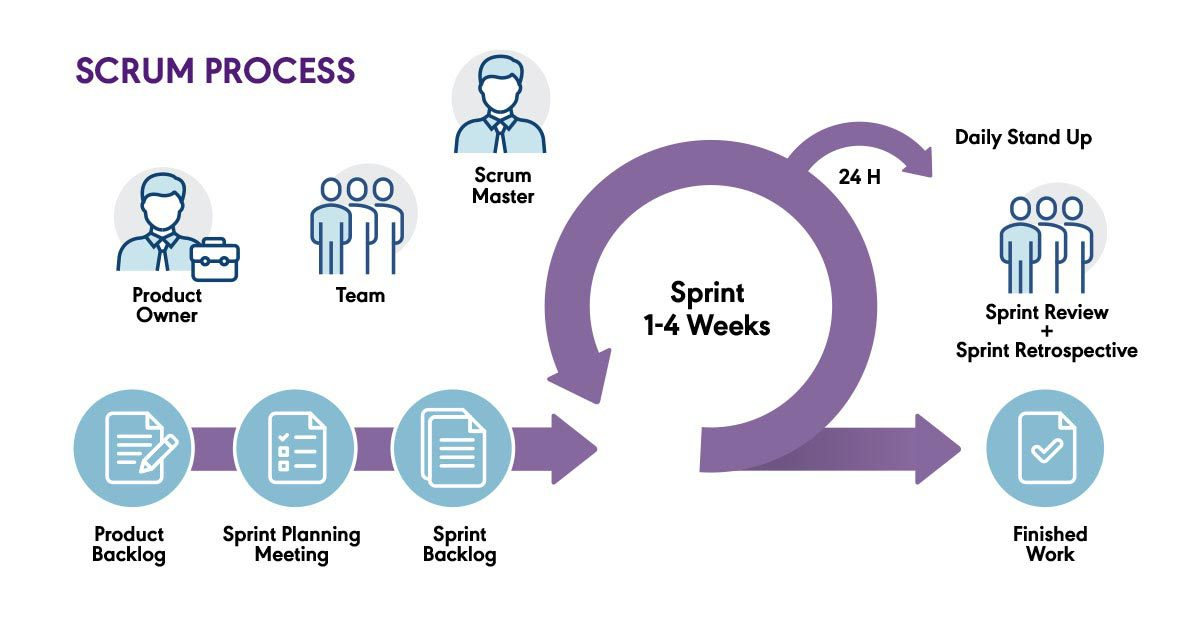
\includegraphics[width=1\textwidth]{images/scrum_process_diagram.jpg}
    \caption{Scrum development process}
    \label{fig:scrum_process}
\end{figure}

As illustrated in Figure~\ref{fig:scrum_process}, Scrum defines three main roles:
\begin{itemize}
  \item \textbf{Product Owner:} Represents the client’s vision and business goals. Defines priorities and validates deliverables.
  \item \textbf{Scrum Master:} Facilitates Scrum processes, ensures the team adheres to the framework, and removes impediments.
  \item \textbf{Development Team:} Executes the technical tasks required to implement features defined in the sprint backlog.
\end{itemize}

\subsection{Project Team and Role Assignment}

The project was carried out by a small but efficient team, where each member was assigned a distinct Scrum role, as detailed in Table~\ref{tab:scrum_roles}. This clear separation of responsibilities enabled smooth collaboration and effective project tracking.

\begin{table}[H]
    \centering
    \begin{tabularx}{\textwidth}{|X|X|X|}
        \hline
        \textbf{Role} & \textbf{Responsibilities} & \textbf{Assigned Member} \\
        \hline
        Product Owner & Defines the product features and validates sprint deliverables & Salah Werda \\
        \hline
        Scrum Master & Oversees project progress and supports the development team & Youssef Aouadni \\
        \hline
        Development Team & Implements user stories and delivers sprint goals & Houcem Chhaidar \\
        \hline
    \end{tabularx}
    \caption{Scrum Roles and Assigned Team Members}
    \label{tab:scrum_roles}
\end{table}

\subsection{Product Backlog}

The product backlog consists of a prioritized list of all functionalities, technical tasks, and improvements needed for the final version of the Credix application. It serves as a dynamic roadmap, regularly updated throughout the project lifecycle.

Sprint planning was conducted at the beginning of each iteration to break down the backlog into manageable chunks, each aligned with a specific sprint objective. In our case, we opted for four-week sprints to balance delivery pace with the opportunity for refinement and feedback.

Each sprint included a selection of user stories—descriptions of product features from an end-user perspective—that were further broken down into technical tasks assigned to team members. This approach ensured both transparency and traceability of progress across the development lifecycle.

\subsection{Sprint Planning}

Prior to the core development cycle, we conducted a two-week preliminary phase commonly referred to as a \textbf{Sprint 0}. This initial sprint was dedicated to project setup and team onboarding, and included the following activities:

\begin{itemize}
    \item Environment setup: installation and configuration of Flutter SDK, JDK, MongoDB, and Spring Boot dependencies.
    \item Initialization of the Git repository with clear branching strategy and commit conventions.
    \item Configuration of CI/CD pipelines using GitHub Actions for both frontend and backend components.
    \item Technical onboarding and knowledge-sharing sessions on key technologies: Flutter, Spring Boot, and the BLoC pattern.
\end{itemize}

Sprint 0 established a solid technical foundation but is not included in the four main development sprints outlined below. Each of the subsequent sprints had a duration of four weeks and was concluded with a sprint review to demonstrate deliverables, gather feedback, and plan improvements for the following iteration.

\vspace{1em}
\begin{longtable}{|p{3cm}|p{10cm}|p{2cm}|}
\caption{Sprint breakdown and objectives \label{tab:sprint_plan}}\\
\hline
\textbf{Sprint} & \textbf{Main Objectives} & \textbf{Duration} \\
\hline
\endfirsthead

\multicolumn{3}{c}%
{{\bfseries \tablename\ \thetable{} -- continued from previous page}} \\
\hline
\textbf{Sprint} & \textbf{Main Objectives} & \textbf{Duration} \\
\hline
\endhead

\hline \multicolumn{3}{r}{{Continued on next page}} \\
\endfoot

\hline
\endlastfoot

\textbf{Sprint 1} & 
\begin{itemize}
  \item Secure authentication (registration, login, JWT)
  \item Role-based access for End-User, Vendor, Corporate
  \item Biometric auth integration (Flutter)
  \item Wallet balance + transaction view
\end{itemize}
& 4 weeks \\
\hline

\textbf{Sprint 2} & 
\begin{itemize}
  \item Barcode payment + validation API
  \item POS integration and fraud detection rules
  \item Offline mode for POS/mobile
  \item Payment confirmation logic
\end{itemize}
& 4 weeks \\
\hline

\textbf{Sprint 3} & 
\begin{itemize}
  \item Corporate portal: credit purchase, employee management
  \item Dynamic credit distribution and spending limits
  \item Fraud engine: frequency checks and freezing
  \item Multi-language support (EN/FR/AR)
\end{itemize}
& 4 weeks \\
\hline

\textbf{Sprint 4} & 
\begin{itemize}
  \item Vendor portal: settlements, POS reports
  \item OTP for high-value payments
  \item CI/CD pipelines and SonarQube
  \item Reporting: CSV/PDF downloads
\end{itemize}
& 4 weeks \\
\hline

\end{longtable}
\vspace{1em}

\subsection{Project Breakdown by Releases}

To align with Scrum methodology, the project is structured into two releases, each covering two sprints of four weeks:

\begin{itemize}[nosep]
  \item \textbf{Release 1}: covers Sprints 1 and 2, focusing on user authentication, wallet and transaction features, and payment validation logic.
  \item \textbf{Release 2}: covers Sprints 3 and 4, dedicated to the corporate and vendor portals, reporting features, multi-language support, and CI/CD pipelines.
\end{itemize}

\begin{figure}[htbp]
  \centering
  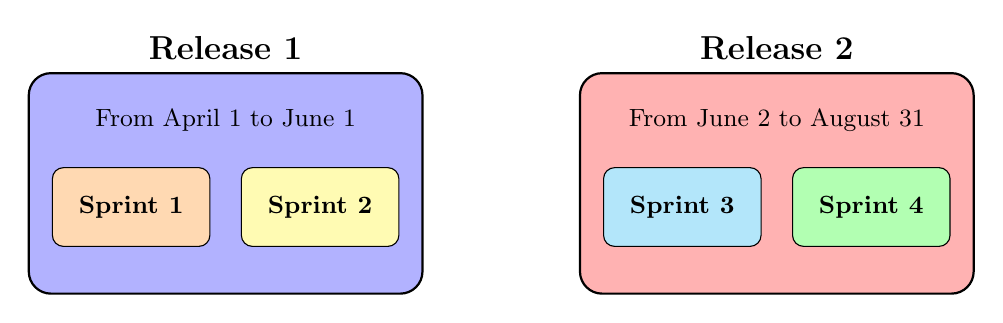
\begin{tikzpicture}[
    box/.style={draw, thick, rounded corners=8pt, minimum width=5cm, minimum height=2.8cm, inner sep=8pt},
    sprintOrange/.style={draw, fill=orange!30, rounded corners=4pt, minimum width=2cm, minimum height=1cm, align=center, font=\small\bfseries},
    sprintYellow/.style={draw, fill=yellow!30, rounded corners=4pt, minimum width=2cm, minimum height=1cm, align=center, font=\small\bfseries},
    sprintCyan/.style={draw, fill=cyan!30, rounded corners=4pt, minimum width=2cm, minimum height=1cm, align=center, font=\small\bfseries},
    sprintGreen/.style={draw, fill=green!30, rounded corners=4pt, minimum width=2cm, minimum height=1cm, align=center, font=\small\bfseries}
  ]
  
  % Release 1
  \node[box, fill=blue!30] (r1) at (0,0) {};
  \node at (r1.north) [yshift=0.3cm, font=\bfseries\large] {Release 1};
  \node at (r1.center) [yshift=0.8cm, font=\small] {From April 1 to June 1};
  \node[sprintOrange] at ([xshift=-1.2cm, yshift=-0.3cm]r1.center) {Sprint 1};
  \node[sprintYellow] at ([xshift=1.2cm, yshift=-0.3cm]r1.center) {Sprint 2};
  
  % Release 2
  \node[box, fill=red!30] (r2) at (7,0) {};
  \node at (r2.north) [yshift=0.3cm, font=\bfseries\large] {Release 2};
  \node at (r2.center) [yshift=0.8cm, font=\small] {From June 2 to August 31};
  \node[sprintCyan] at ([xshift=-1.2cm, yshift=-0.3cm]r2.center) {Sprint 3};
  \node[sprintGreen] at ([xshift=1.2cm, yshift=-0.3cm]r2.center) {Sprint 4};
  
  \end{tikzpicture}
  \caption{Project Releases Timeline}
  \label{fig:releases_tikz}
\end{figure}

\subsection{Work Planning Tool}

To effectively apply the Scrum methodology during the development of this project, I used \textbf{Jira}. This platform enabled me to organize, monitor, and manage the work in an Agile manner while maintaining a clear workflow structure. Jira is one of the most popular tools for Agile project management. It provides a robust environment where tasks can be linked to user stories, sprints, and the product backlog, allowing efficient tracking of each item throughout its lifecycle.

One of Jira’s key features is the \textbf{Kanban board}, which offers a collaborative workspace for managing sprint workflows. It allows visual tracking of progress, priority setting, and improved clarity on task ownership and sprint structure.

\begin{figure}[H]
  \centering
  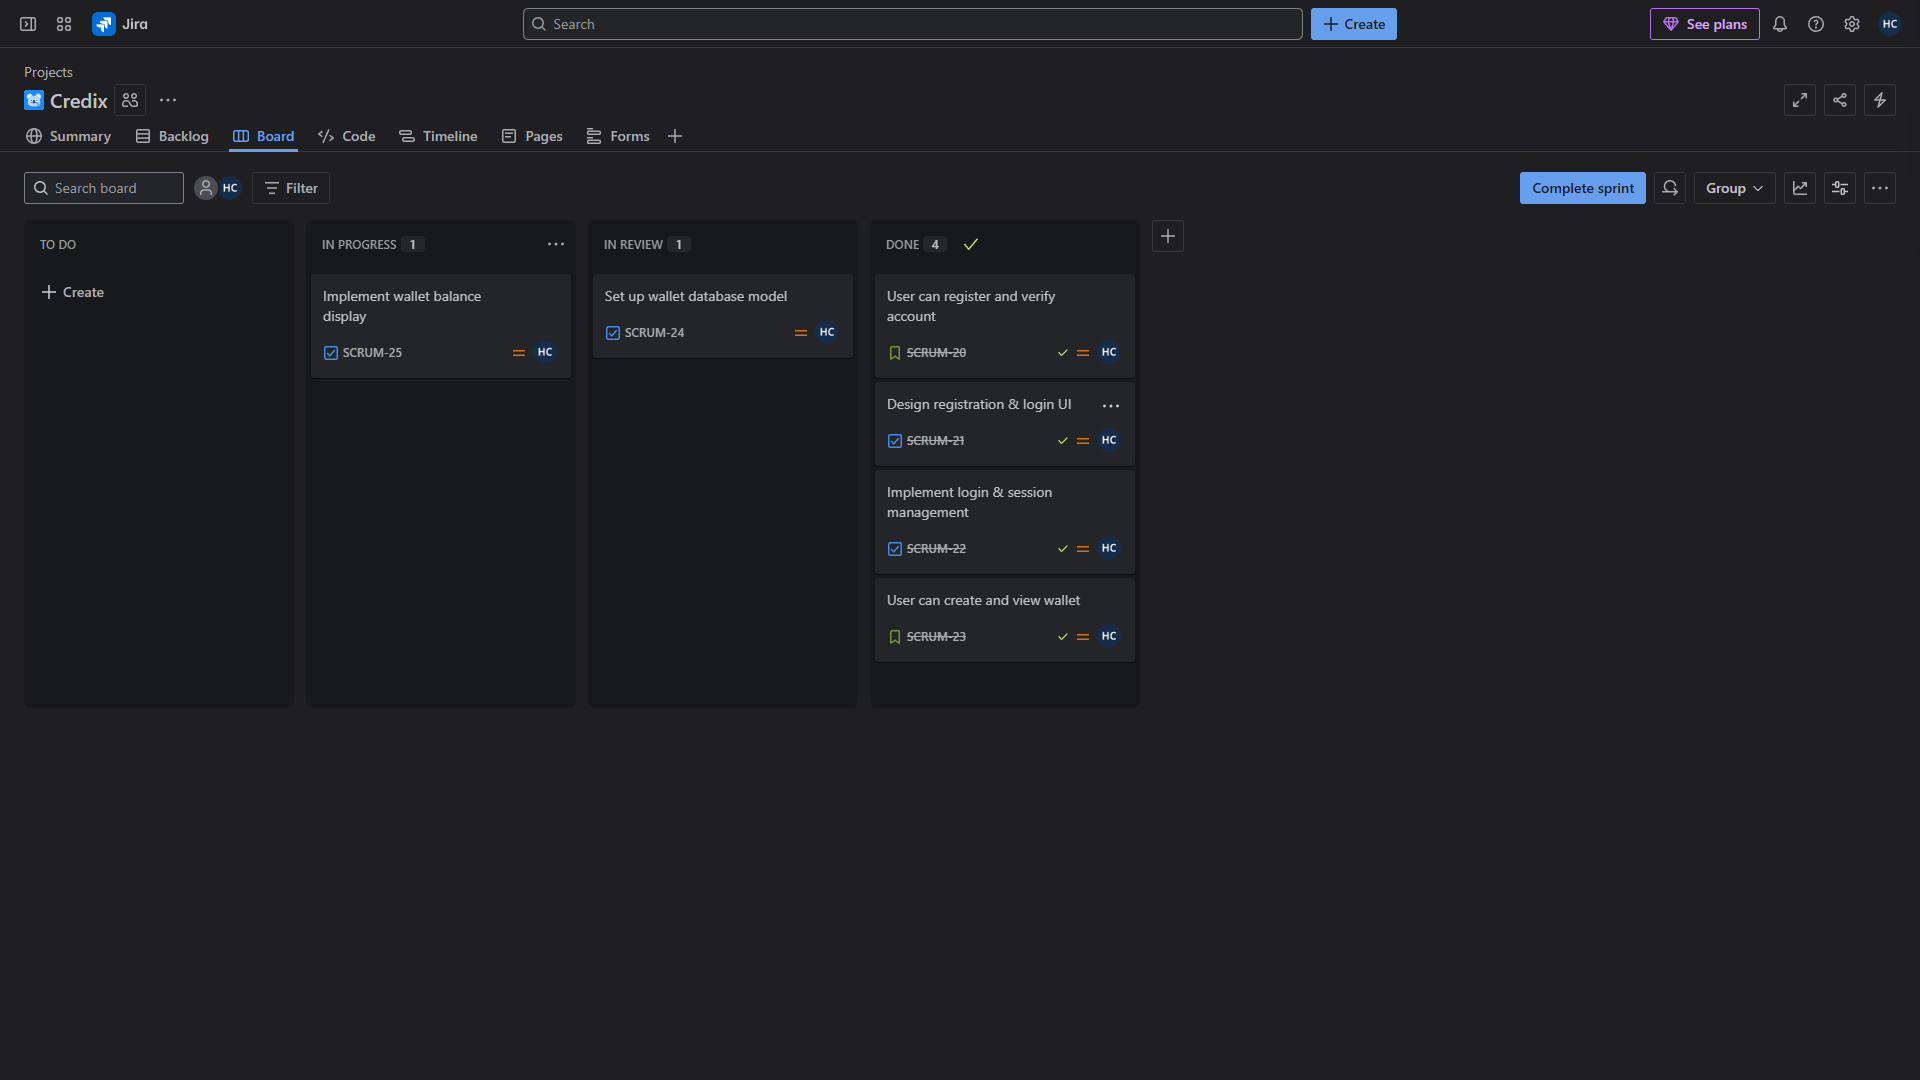
\includegraphics[width=\textwidth]{images/jira_board_sprint_1.png}
  \caption{Jira board snapshot for Sprint 1}
  \label{fig:jira_board_sprint1}
\end{figure}

Figure~\ref{fig:jira_board_sprint1} presents an extract from the first sprint’s board on Jira. This view highlights how the tool was used to define, categorize, and track tasks across different stages of the sprint. Each task was associated with a user story, assigned a priority, and monitored throughout its lifecycle, ensuring traceability and alignment with sprint objectives.

By leveraging Jira’s functionalities, such as task assignment, deadline management, and progress visualization, it was possible to maintain rigorous sprint planning and execution. The tool also supported the identification of bottlenecks, facilitated real-time adjustments, and ensured that the project milestones were met in accordance with the defined timeline and Agile principles.

